

\section{Reduction through Lifetime}

Conventionally 



\subsubsection{Calculating the lifetime}
Within models a species lifetime is regarded as the time taken for its concentration to halve [ref]. This works on the assumption that the species is not produced, and that rate coefficients and other constants remain constant. For a first order decay of sample \autoref{eqn}, we can represent the decay using \autoref{decay}, showing that the half life is independent of initial concentration. 

\begin{equation}
A \rightarrow{^k} B
\label{eqn}
\end{equation}

\begin{equation}
s(t) = a_0 \exp(-kt) \\
\frac{a(t)}{a_0} = \exp(-kt) \\
$$linearised this gives$$
\ln (\frac{a(t)}{a_0}) = -kt
$$ after $\tau_{1/2}$ the concentration is equal to $a_0/2$ of initial rate $a_0$, which gives $$
\ln(\frac{\frac{a_0}{2}}{a_0}) = \ln(\frac{1}{2}) = \ln(2^{-1}) = -\ln2 = k\tau_{1/2} 
$$$$
\tau_{\frac{1}{2}} = \frac{\ln 2}{k}
\label{decay}
\end{equation}

In species of the first order only, this may simplified to 
\begin{equation}
a(t) = a_0 \exp (t  \sum_j k_j )
$$ and therefore the half life may be written as the reciprocal sum of rate coefficients: $$
\tau_A = 1 / \sum_j k_j
\end{equation}

and is how lifetime is calculated for photochemical species [ref! pillin and seakins]. An alternative method for half life calculation may be obtained using the diagonal (self reference) of a Jacobian matrix ,\cite{kinetics}:

\begin{equation}
\tau_1 = - \frac{1}{J_{ii}}
\end{equation} 

This value will usually be negative unless a species does not contain a consuming reaction, then it will be zero. 


The xxxxx method of reduction consists of the isolation of species with similar lifetimes and reactions as a means of lumping. In doing so the ... etc 


\subsection{Comparing Magnitude and Direction}
Since the photolysis reactions in a model change the resultant rates, and thus flux of a species depending on the azimuthal angle related to the time of day, we not only want to compare species with the same magnitude, they also need to match the profile as they change. To do this we may represent all pariwise species matches on a latent space representing the size and angle between their temporal vectors. This is done through using the euclidean distance on the $x$ axis, and cosine distance $y$ on the $y$. 

\subsubsection{Euclidian distance}
This is the simplest method of vector comparison and works by calculating the distance between all points in two vectors. For the vectors

\begin{equation}
v1 = [ a,b,c, \dots n ] 
$$$$
v2 = [ i,j,k, \dots z ]
\end{equation}

This can be done using pythoagoras' theorem in \autoref{euclid}:

\begin{equation}
e_{dist}  = \sqrt{(a-i)^2 + (b-j)^2 + (c-k)^2 + \dots + (n-z)^2}
\label{euclid}
\end{equation}

This transformation converts the straight line distance between each vector into metric space, allowing us to represent the difference in their magnitudes as a single scalar. Unfortunately as this requires the difference between all permutations of rows, it cannot be done as a single operation, but as multiple. \\

APPLICA"tiion

\subsubsection{Cosine Distance} 

Similarly if we wish to calculate the angle between two vectors we may use the cosine difference. In starting with the definition of the dot product 

\begin{equation}
v1 \cdot v2 = \|v1\|\|v2\| \cos \theta
$$this may be arranged$$
\cos \theta = \frac{ v1 \cdot v2}{\|v1\|\|v2\|}
\end{equation}

Since this does not work for the triangle ? inequality, we need to normalise each vector before calculating the cosine distance. The merits of this come from  ... which makes its application comparing the similarity between texts or documents of different sizes very popular (REF!). \\



\subsection{Temporal Lifetime Vector Comparison}

To compare a species diurnal profile with its absolute lifetime we can plot the cosine and eudlidian distance against eachother. In this subsection compute the euclidean and cosine distances for all remaining reaction pairs (88410 pairs) for a single simulation. We start by looking that the species density profiles, \autoref{fig:density2}. Here we can see that most of the species within our mechanism fall under two peaks. The first is a peak of great similarity between pairs of species (close to 1), where both the diurnal profile and concentration differences change simultaniously, The other contains species with a simiar dirunal profiles, that do not change at the same rate as eachotehr. In general the euclidean distances are smaller than the cosine distances, suggesting a greater concenration change between pairs of species with the same profile. 



\begin{figure}
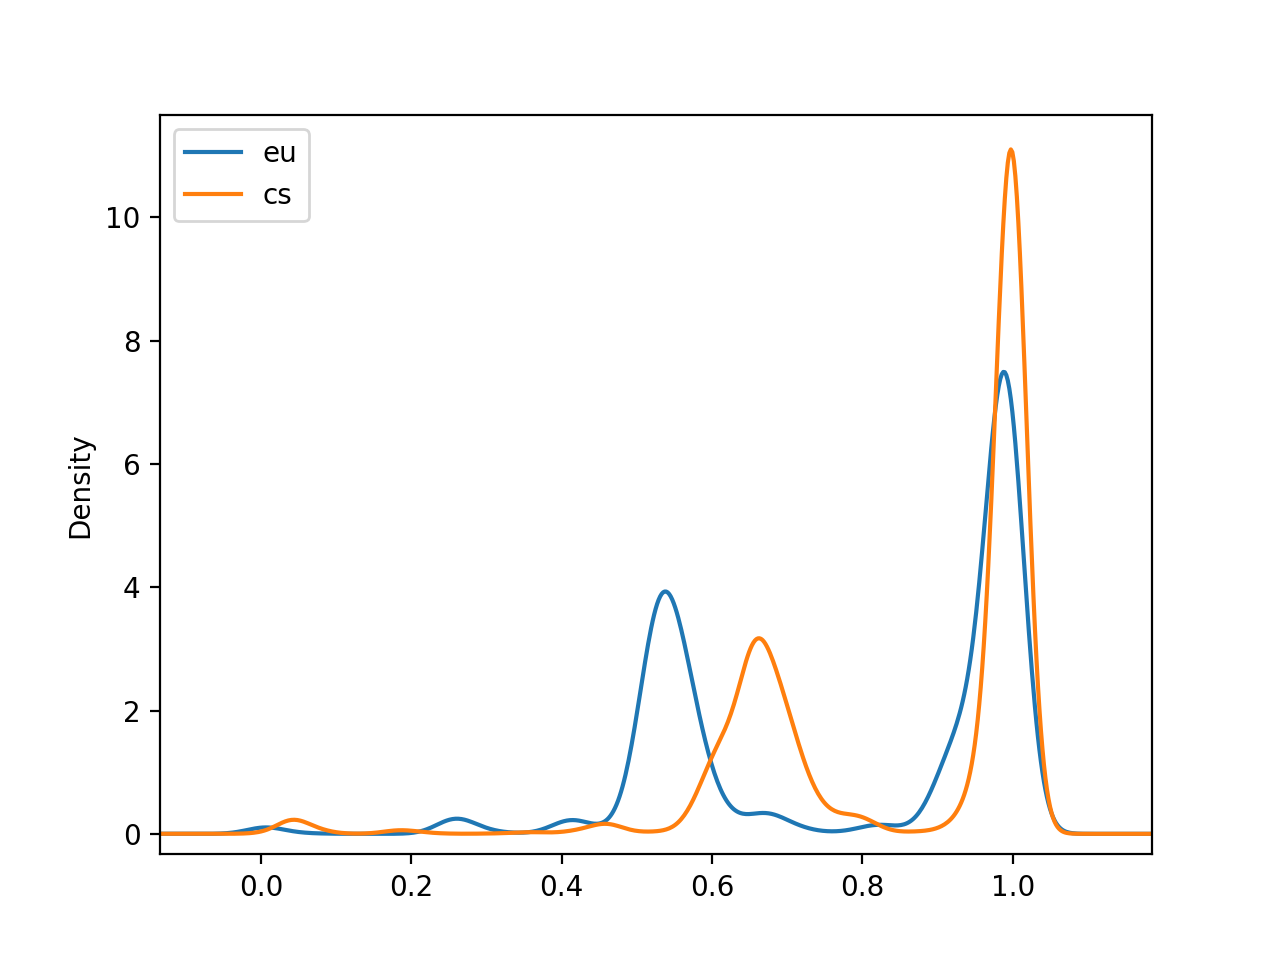
\includegraphics[width=.7\textwidth]{fig/metric_density.png}
\caption{Gaussian Kernel Density Estimate plot showing the distributions present for the \{0,1\} scaled euclidean and cosine distances.}
\label{fig:density2}
\end{figure}



and plot them on separate axis, \autoref{fig:morig}. Here the colour represents the geometric mean of both normalised values. Due to the large number of 




Since there are $n^2$ different combinations, this process can be lengthy to compute. Moreover the number of nodes present makes it difficult to visually determine which couplets to lump together, especially when they are overlaying eachother, as in \autoref{fig:metric}. To overcome this we apply a force graph simulation to each node. Here a strong force pulls them towards their true location, whist a collision/repulsive force ensures that there exists no overlap between nodes. Although some information loss may be incurred this way, it does enable us to interactively determine which pairs belong to which points.   

Plotting the data this way provides an approximate view of how lifetimes change within the system. \autoref{fig:density2} shows the distribution of values across both metrics. Here we see that although there is some difference the cosine difference can be used as an indicator for exploring further. This is useful since the cosine difference is a matrix operation and can produce near instant results in the form of the output relationship matrix. The euclidean distance however must be computed for each coupling individually as it requires taking the difference between the temporal lifetime arrays of each species. This means that rather than computing the euclidean distance for all permutaions of species, we can compute only those whose cosine distances suggest potentially promising results.  



\begin{figure}[H]
\begin{subfigure}{.5\textwidth}
  \centering
  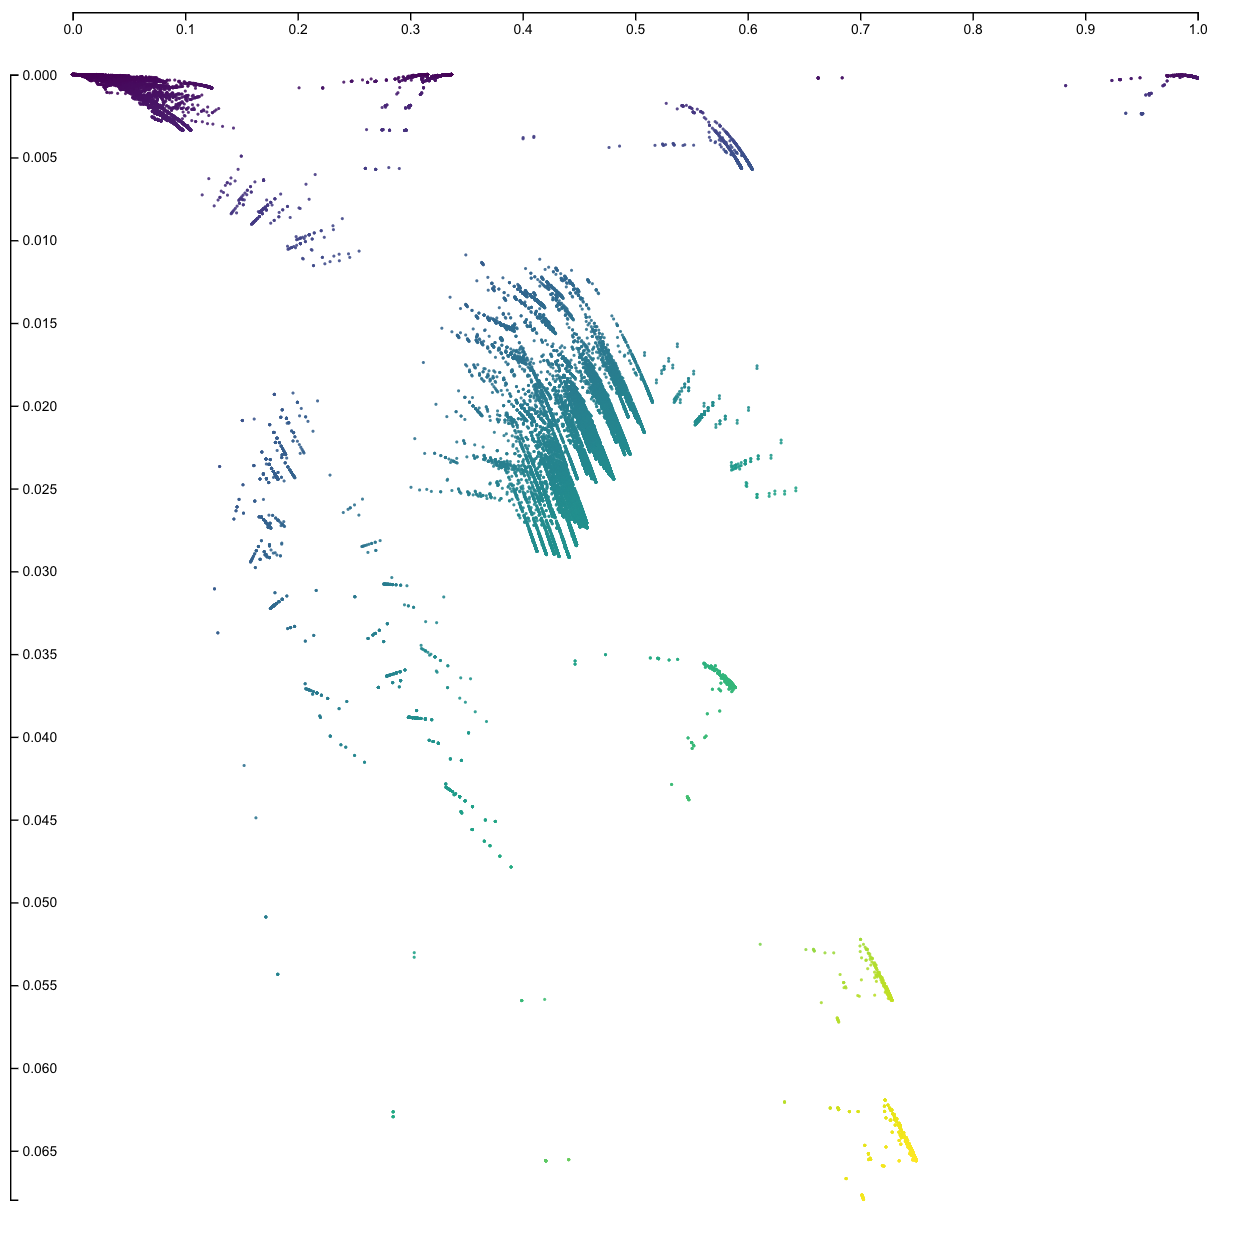
\includegraphics[width=\textwidth]{fig/metric-1.png}
  \label{fig:morig}
  \caption{Original}
\end{subfigure}%
\begin{subfigure}{.5\textwidth}
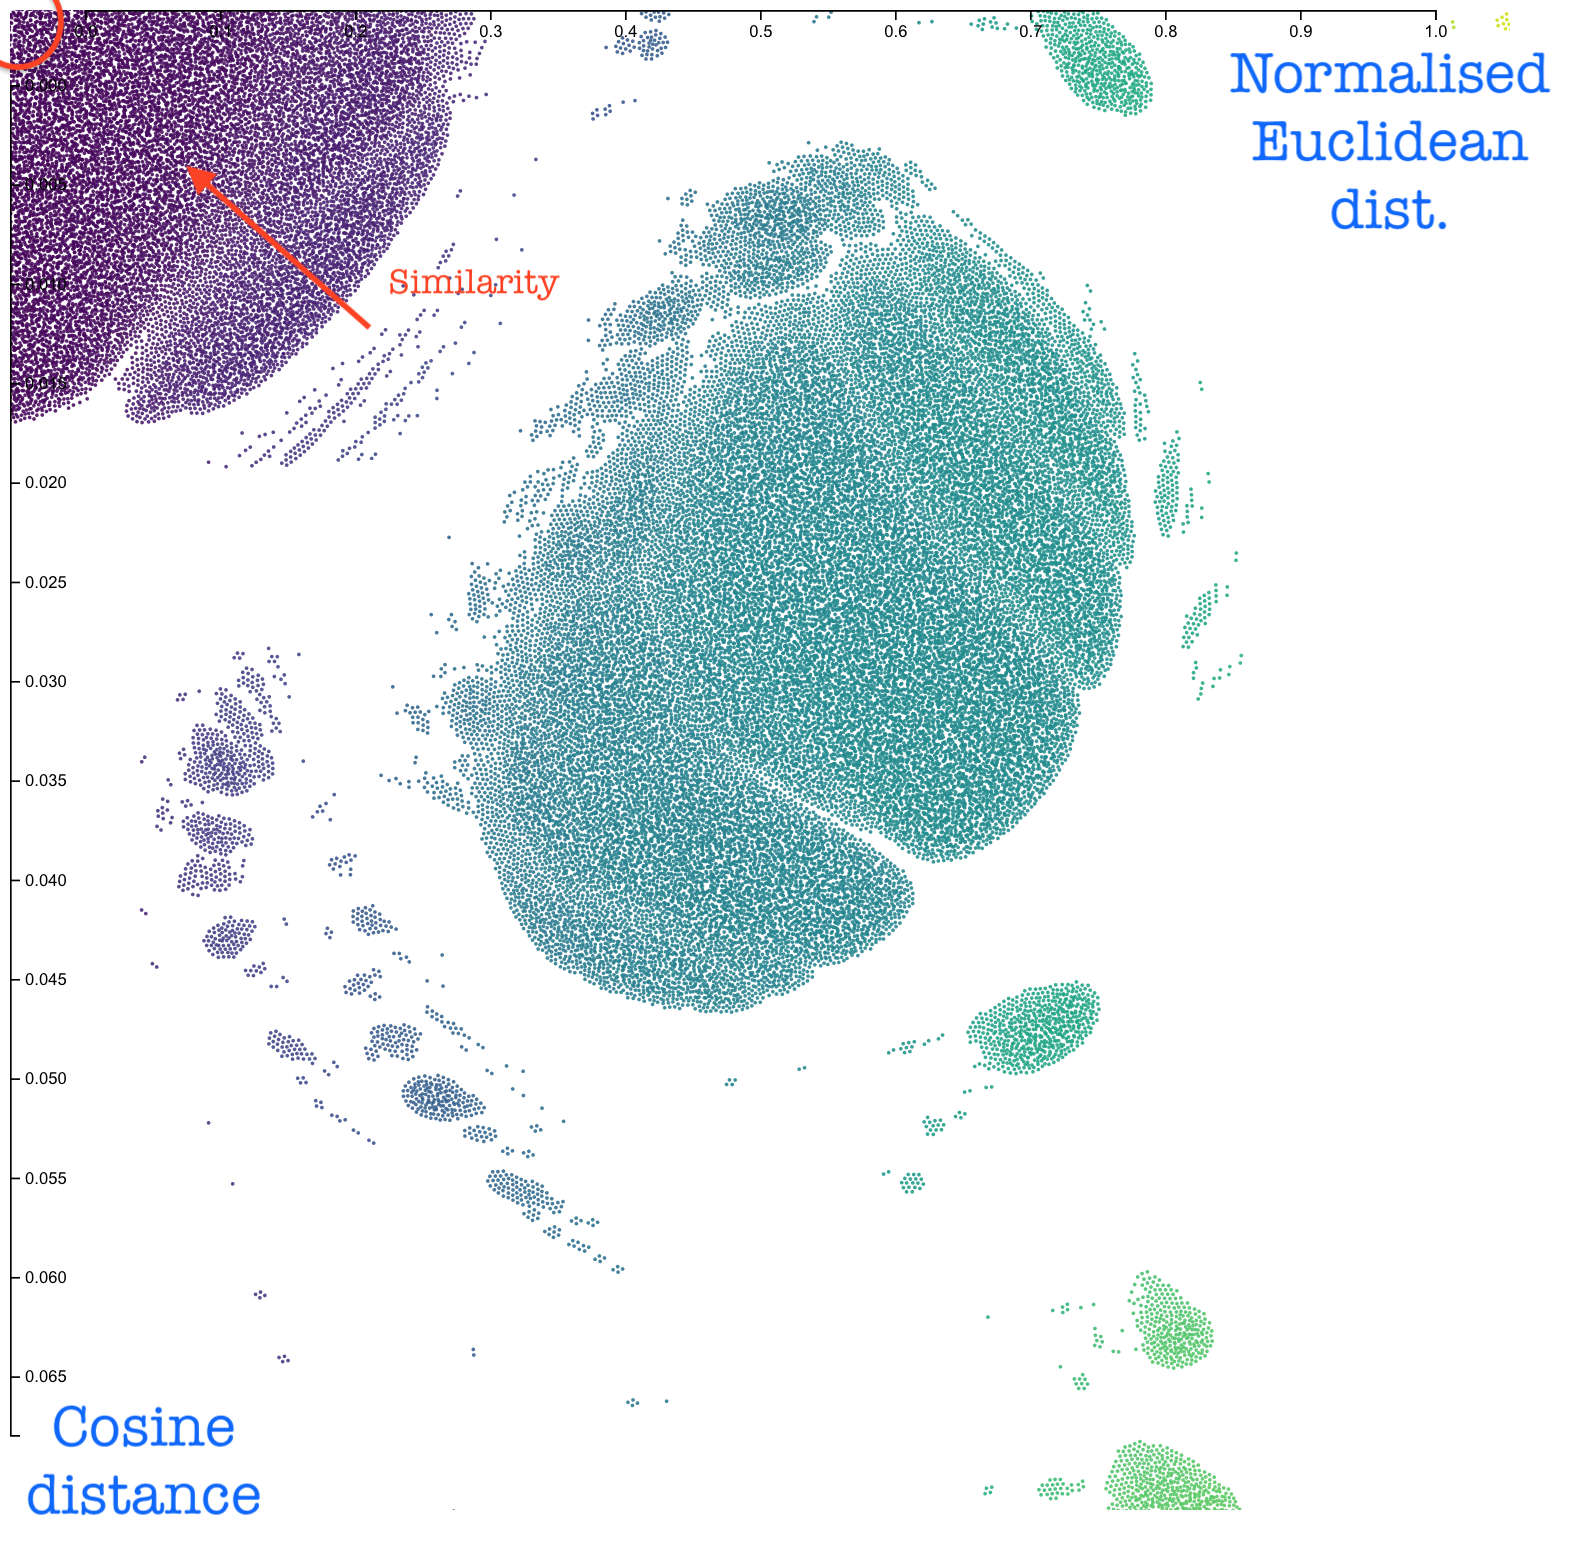
\includegraphics[width=\textwidth]{fig/metric.png}
\label{fig:metric}
\caption{Interactive, non overlapping plot of normalised euclidian distance across the x axis against the cosine distance on the y. The colouring is the geometric mean between them.}
\end{subfigure}

\caption{Showing the evolution from the original overlaid locations, \autoref{fig:morig} to the slightly more accessible (interactively) \autoref{fig:metric}}
\end{figure}

